% -*- LaTeX -*-
% -*- coding: utf-8 -*-
%
% ~~~~~~~~~~~~~~~~~~~~~~~~~~~~~~~~~~~~~~~~~~~~~~~~~~~~~~~~~~~~~~~~~~~~~~~~~~~~~~
%
%                             michael a.g. aïvázis
%                      california institute of technology
%                      (c) 1998-2010  all rights reserved
%
% ~~~~~~~~~~~~~~~~~~~~~~~~~~~~~~~~~~~~~~~~~~~~~~~~~~~~~~~~~~~~~~~~~~~~~~~~~~~~~~
%

\lecture{Unstructured grids}{20100222}

% --------------------------------------
% overview of unstructured grids
\begin{frame}[fragile]
%
  \frametitle{Unstructured grids}
%
  \begin{itemize}
%
  \item solving differential equations using structured grids
    \begin{itemize}
    \item finite differences
    \item finite volumes
    \end{itemize}
%
  \item finite elements take a different approach
    \begin{itemize}
    \item subdivide the domain into elements
    \item construct basis functions over each element
    \item 
    \end{itemize}
%
  \item a {\em simplicial mesh}
%
  \item what follows is an overview of very common but surprisingly hard problems that occur in
    simulations of physical systems
  \end{itemize}
%
\end{frame}

% --------------------------------------
% overview of unstructured grids
\begin{frame}[fragile]
%
  \frametitle{Finite elements}
%
  \begin{itemize}
%
  \item 
%
  \item 
%
  \end{itemize}
%
\end{frame}

% --------------------------------------
% meshing
\begin{frame}[fragile]
%
  \frametitle{Meshing}
%
  \begin{itemize}
%
  \item creating simplicial meshes is a surprisingly hard problem
%
  \item in two dimensions
    \begin{itemize}
    \item there is a well posed mathematical problem with some guarantees that a triangulation
      can be generated for sufficiently well defined domains
      \begin{itemize}
      \item given a set of vertices, one can always find a {\em Delaunay} triangulation where
        no vertex falls in the interior of the circumcircle of any triangle
      \item the quality of the triangulation can be improved by adding extra vertices
      \end{itemize}
    \item for practical purposes, this is sufficient to handle most cases
    \item the problem is rather challenging numerically, with high incidence of round-off
      errors, overflows and underflows
      \begin{itemize}
      \item certain geometrical tests are so sensitive that robust packages employ exact
        arithmetic
      \end{itemize}

    \end{itemize}
%
  \item similar guarantees exist when triangulating surfaces embedded in three dimensional
    space
%
  \item in three dimensions the problem is theoretically intractable at this point
    \begin{itemize}
    \item meshing packages are full of heuristics to avoid the known pathological cases
    \end{itemize}
%
  \item no known parallel implementations 
%
  \end{itemize}
%
\end{frame}

% --------------------------------------
% overview of unstructured grids
\begin{frame}[fragile]
%
  \frametitle{Parallelization}
%
  \begin{minipage}{.80\linewidth}
%
    \begin{itemize}
%
    \item typically, the finest grain task is the element update that models the response of the
      material to the deformation induced by the motion of the vertices
      \begin{itemize}
      \item that's where all the physics is
      \item computationally intensive for non-trivial responses
        \begin{itemize}
        \item usually involves solving a complicated variational problem, such as energy
          minimization
        \end{itemize}
      \item little or no interaction with neighboring elements, although non-local updates are
        becoming more common
        \begin{itemize}
        \item e.g.~thin shells, fracture based on deformation energy in a neighborhood
        \end{itemize}
      \end{itemize}
%
    \item coarse grain tasks are defined through {\em graph partitioning} that decomposes the
      mesh into smaller subgraphs
      \begin{itemize}
      \item with uniform element and node distributions
      \item well characterized boundaries
      \end{itemize}
% 
    \item performance characteristics
      \begin{itemize}
      \item computational cost grows with the number of elements
      \item communication cost grows with the number of nodes on partition boundaries
      \end{itemize}
%
    \end{itemize}
%
  \end{minipage}
%
  \hfill
  \begin{minipage}{.17\linewidth}
    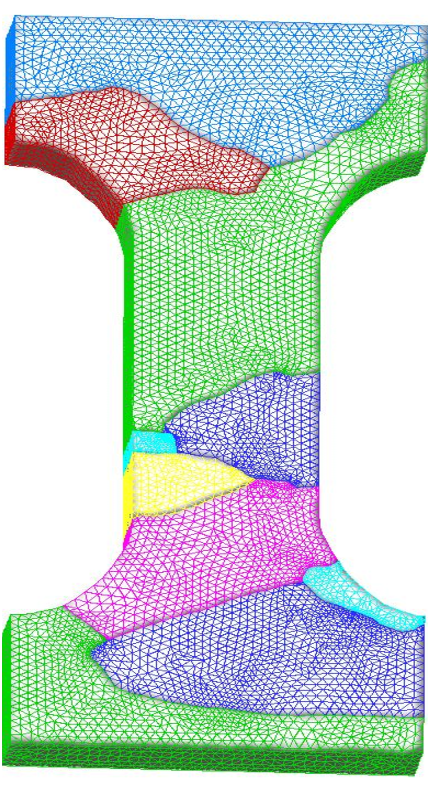
\includegraphics[scale=0.3]{figures/mesh-dogbone.pdf}
  \end{minipage} 
%
\end{frame}

% --------------------------------------
% graph partitioning
\begin{frame}[fragile]
%
  \frametitle{Graph partitioning}
%
  \begin{itemize}
%
  \item mesh domain decomposition is mathematically identical to graph partitioning
    \begin{itemize}
    \item a {\em hard} computational problem
    \item with wide applicability to many practical problems
    \item hence, there are many excellent algorithms -- and software packages -- that solve
      most problems of practical interest
    \end{itemize}
%
  \item algorithms fall into two broad categories
    \begin{itemize}
    \item those that use geometrical information, such as nodal co\"ordinates
    \item those that rely only on graph connectivity
      \begin{itemize}
      \item breadth first search, spectral bisection, Kernighan/Lin
      \end{itemize}
    \end{itemize}
%
  \item comparison metrics
    \begin{itemize}
    \item speed of partitioning: important since meshes tend to be large
    \item number of cut edges
    \item for finite elements: important to minimize the number of nodes on partition
      boundaries, since it is directly linked to the communication cost of the calculation
    \end{itemize}
%
  \item METIS from George Karypis' lab at the University of Minnesota
    \begin{itemize}
    \item multi-level Kernighan/Lin algorithms, other heuristics
    \item ParMETIS is the parallel implementation
    \end{itemize}
%
  \end{itemize}
%
\end{frame}

% --------------------------------------
% uniform subdivision
\begin{frame}[fragile]
%
  \frametitle{Uniform subdivision}
%
  \begin{itemize}
%
  \item high fidelity simulations require high resolution
    \begin{itemize}
    \item i.e.~small elements, which implies large element counts
    \item many interesting problems require tens or hundreds of millions of elements before
      they converge
    \item creating input meshes of this size sequentially is impractical
    \end{itemize}
%
  \item one possibility is {\em parallel uniform subdivision}
    \begin{itemize}
    \item the input mesh is partitioned and distributed among processes
    \item each process subdivides its simplices
      \begin{itemize}
      \item edges get split in two, triangles in four, tetrahedra in eight
      \item mesh quality is not affected significantly: only two new classes of simplices are
        introduced, regardless of the number of subdivision levels
      \item the formation of new entities on partition boundaries implies the recalculation of
        the communications maps among processes
      \end{itemize}
    \end{itemize}
%
  \begin{minipage}{.6\linewidth}
    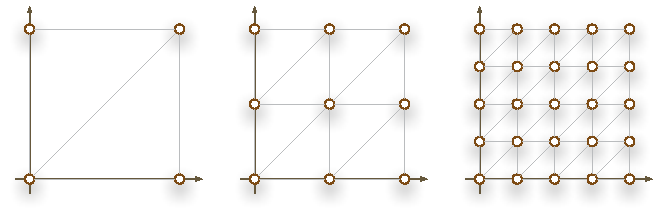
\includegraphics[scale=0.5]{figures/mesh-subdivision.pdf}
  \end{minipage}
    \hfill
  \begin{minipage}{.35\linewidth}
    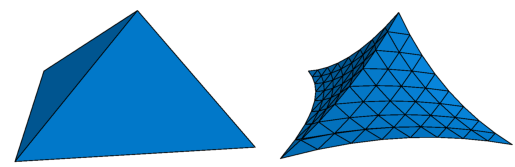
\includegraphics[scale=0.5]{figures/mesh-tetsubdivision.pdf}
  \end{minipage}
%
  \item can be done in linear time
    \begin{itemize}
    \item scales well and can create enormous meshes (billions of elements)
    \end{itemize}
%
  \end{itemize}
%
\end{frame}

% --------------------------------------
% non-uniform subdivision
\begin{frame}[fragile]
%
  \frametitle{Non-uniform subdivision and adaptive remeshing}
%
  \begin{itemize}
%
  \item there are many good non-uniform subdivision algorithms
    \begin{itemize}
    \item e.g.~longest edge subdivision: each tetrahedron that has an edge longer than some
      threshold gets subdivided by splitting that edge in two and connecting the new node to
      the two non-adjacent vertices
    \end{itemize}
%
  \item they tend to be difficult to parallelize because they induce {\em one-sided}
    topological changes on the partition boundaries that must be communicated to the
    neighboring process
    \begin{itemize}
    \item hence they are rarely used in large scale calculations
    \item this is  an {\em architectural} limitation, not an {\em algorithmic} one!
    \item it requires restructuring the solver to support non-trivial communication with its
      neighbors
    \end{itemize}
%
  \item similar considerations apply to adaptive remeshing
    \begin{itemize}
    \item where a process discovers that it requires a higher element density to satisfy some
      correctness criterion
    \item but difficult to implement when the refinement reaches the partition boundary
    \end{itemize}
%
  \end{itemize}
%
\end{frame}

% --------------------------------------
% contact detection
\begin{frame}[fragile]
%
  \frametitle{Contact detection}
%
  \begin{itemize}
%
  \item modeling impact requires detecting when bodies come into contact and computing
    appropriate forces
    \begin{itemize}
    \item both are difficult problems, especially for non-smooth, distributed meshes
    \item the computations involve only elements on the free boundary
    \end{itemize}
%
  \item the element updates and contact search have very different communication patterns
    \begin{itemize}
    \item contact is {\em global}, since any two surface triangles can collide
    \item and it is expensive, since it involves geometrical queries
    \item it is best solved as an auxiliary parallel problem with its own partitioning
      \begin{itemize}
      \item boundary partitioned using geometric criteria, such as axis-aligned cutting planes
      \item requires frequent re-balancing as mesh geometry and topology change
      \end{itemize}
    \end{itemize}
%
  \item in {\em surface driven} contact detection
    \begin{itemize}
    \item the boundary is partitioned and the centers of all the faces are inserted in some
      kind of spatial data structure
      \begin{itemize}
      \item so that coarse calculations about contact candidates can be made efficiently
      \item typically bucket or sparse-bucket arrays that support {\em orthogonal range
          queries} (ORQ)
      \end{itemize}
    \item candidates can be checked pairwise for actual contact using ray-triangle and
      edge-triangle intersection algorithms
    \end{itemize}
%
  \end{itemize}
%
\end{frame}

% --------------------------------------
% volume-based contact detection
\begin{frame}[fragile]
%
  \frametitle{Volume based contact detection}
%
  \begin{itemize}
%
  \item volume based approaches replace the elements on the boundary with equivalent spheres
  \item a variety of geometrical criteria can be used: 
    \begin{itemize}
      \item equivalent volume
      \item diameter determined by the longest edge
    \end{itemize}
% 
  \item contact detection can take place very efficiently using ORQ algorithms
  \item simple spring models resolve the contact forces
    \begin{itemize}
    \item based on simple potentials that take into account the sphere inter-penetration
    \end{itemize}
%
  \end{itemize}
%
  \begin{figure}
    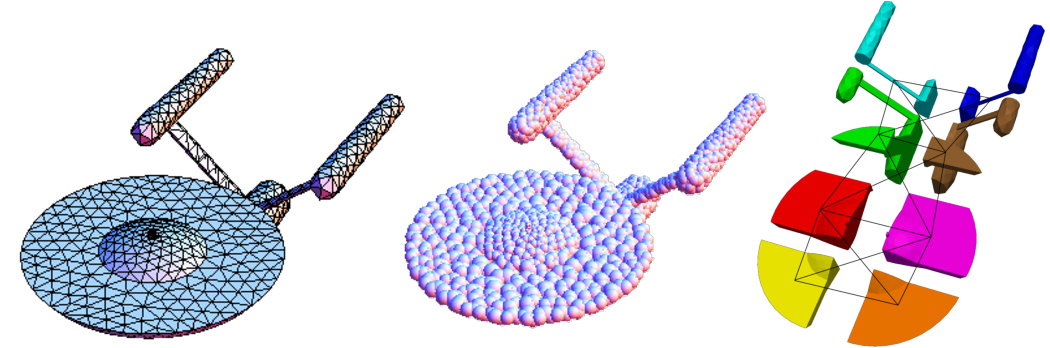
\includegraphics[scale=0.5]{figures/mesh-volumecontact.pdf}
  \end{figure}
%
\end{frame}

% --------------------------------------
% fracture and fragmentation
\begin{frame}[fragile]
%
  \frametitle{Fracture and fragmentation}
%
  \begin{itemize}
%
  \item when the material is under sufficient tension, modeling the physics correctly
    requires topological changes to the mesh
    \begin{itemize}
    \item the material {\em fractures} when it is energetically favorable for an opening to
      form between two elements that are being pulled apart
    \end{itemize}
%
  \item modeling this typically involves {\em cohesive elements}
    \begin{itemize}
    \item prismatic elements that are inserted in the place of what used to be the common face
      of two tetrahedra and absorb excess energy
    \end{itemize}
%
  \item when some threshold is exceeded, the cohesive element fractures and becomes free
    surface
%
  \item cohesive element insertion involves node, edge and face splitting
  \item difficulties arise as cracks run up to process boundaries and must be propagated across
  \item eventually, fragments form as cracks disconnect portions of the mesh
%
  \end{itemize}
%
  \begin{figure}
    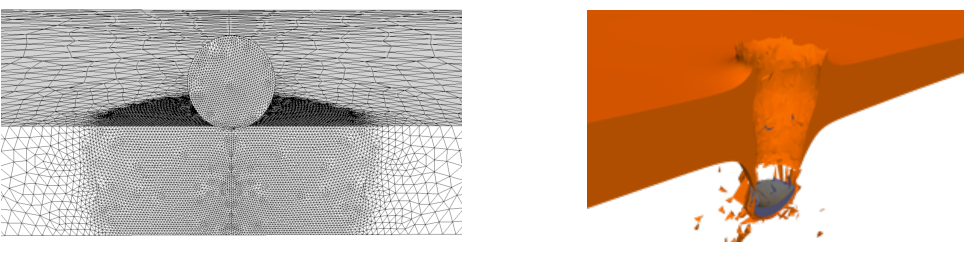
\includegraphics[scale=0.5]{figures/mesh-penetration.pdf}
  \end{figure}
%
\end{frame}

% --------------------------------------
% element erosion
\begin{frame}[fragile]
%
  \frametitle{Element erosion}
%
  \begin{itemize}
%
  \item mesh distortions induced by large deformations
    \begin{itemize}
    \item degrade the numerical accuracy of the calculation
    \item force the timestep sizes to impractical values
    \item eventually cause the simulation to fail
    \end{itemize}
    \begin{figure}
      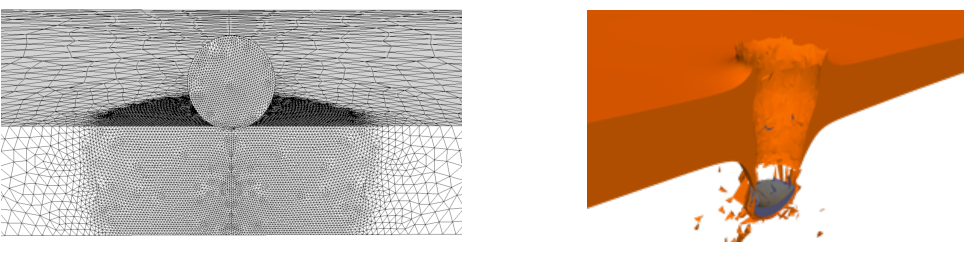
\includegraphics[scale=0.5]{figures/mesh-penetration.pdf}
    \end{figure}
%
  \item a strategy in wide use is to {\em erode} badly distorted elements
    \begin{itemize}
    \item using physically motivated erosion criteria that model fracture mechanics
    \item trivial to implement sequentially
    \item less so in parallel, as it involves geometrical and topological changes to the mesh
    \end{itemize}
%
  \item candidates are selected based on a geometric criterion of the element quality
  \item erosion takes place when the deformation energy in a suitable neighborhood exceeds the
    fracture energy
%
  \end{itemize}
%
\end{frame}

% --------------------------------------
% mesh optimization
\begin{frame}[fragile]
%
  \frametitle{Mesh optimization}
%
  \begin{itemize}
%
  \item the numerical accuracy of finite element calculations is determined in part by the
    quality of the mesh
    \begin{itemize}
    \item the initial triangulation generated by the mesher
    \item distortions induced by large deformations
    \end{itemize}
%
  \item element quality is intuitively related to its deviation from an equilateral tetrahedron
    \begin{itemize}
    \item there are a dozen or so pathological cases that involve either extremely small or
      extremely large internal angles
    \end{itemize}
%
  \item optimizing mesh quality requires
    \begin{itemize}
    \item an element quality metric that places a high penalty on the pathological cases
    \item geometrical optimization: redistributing the mesh nodes so that it is possible to
      construct a defect-free triangulation
    \item topological optimization: adjusting the way nodes are connected to form simplices
    \item control over the element size, which is linked directly to both the numerical
      accuracy and the computational cost of the simulation
    \item a sufficiently well characterized description of the boundary so that when new nodes
      are inserted near the boundary they do not induce distortions
    \end{itemize}
%
  \end{itemize}
%
\end{frame}

% --------------------------------------
% mesh optimization
\begin{frame}[fragile]
%
  \frametitle{Mesh optimization examples}
%
  \begin{itemize}
%
  \item consider a mesh with an embedded sphere that is undergoing rigid rotation
%
  \item a quarter of a turn is sufficient to distort the mesh
    \begin{figure}
      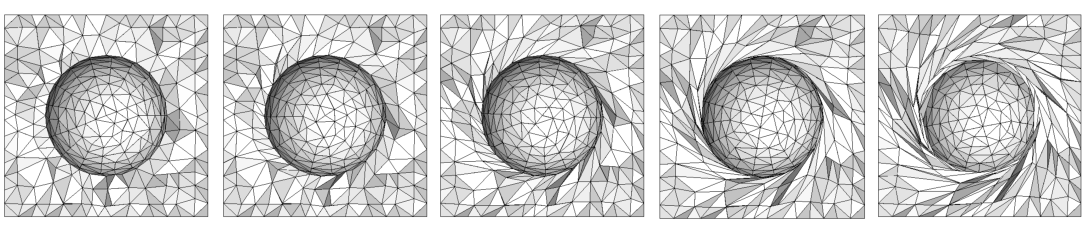
\includegraphics[scale=0.5]{figures/mesh-drag.pdf}
    \end{figure}
%
  \item continuous remeshing maintains good mesh quality; after three whole revolutions
    \begin{figure}
      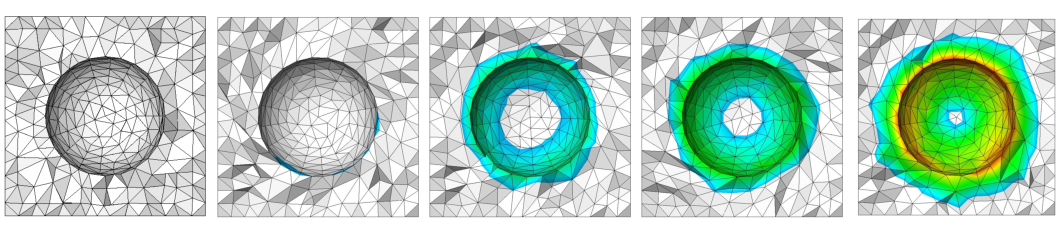
\includegraphics[scale=0.5]{figures/mesh-draghealed.pdf}
    \end{figure}
%
  \item challenges:
    \begin{itemize}
    \item keep numerical diffusion under control
    \item implement in parallel
    \end{itemize}
%
  \end{itemize}
%
\end{frame}

% --------------------------------------
% level sets
\begin{frame}[fragile]
%
  \frametitle{Implicit representations of surfaces}
%
  \begin{itemize}
%
  \item simulating phenomena that involve the interaction of solids and fluids has its own
    challenges
    \begin{itemize}
    \item fluid solvers are typically Eulerian, with structured grid that is fixed in space
      while the fluid flows through it
    \item whereas solid solvers are typically Lagrangian, with an unstructured grid that moves
      along with the body it describes
    \end{itemize}
%
  \item coupling requires some form of information exchange that enables 
    \begin{itemize}
    \item the solid solver to inform the fluid about the position and velocity of its evolving
      boundary
    \item the fluid solver to exert a force on the solid through its pressure field on the
      boundary
    \end{itemize}
%
  \item the solution involves constructing {\em level sets}, and computing the distance to the
    solid, the closest node and the closest face for each point on the grid
%
  \end{itemize}
%
  \begin{figure}
    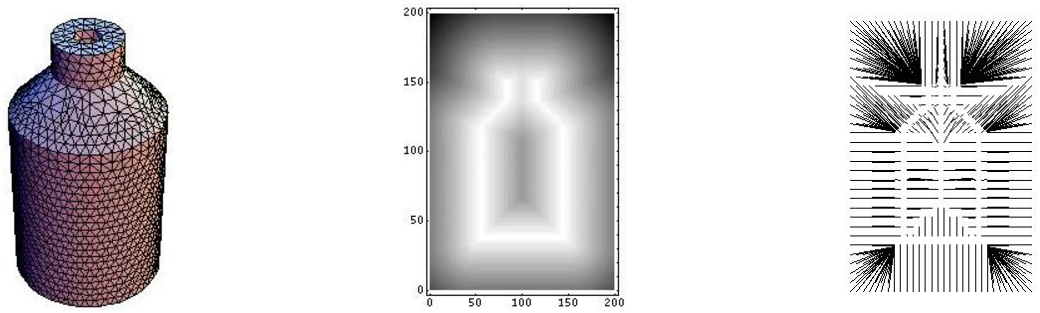
\includegraphics[scale=0.4]{figures/mesh-cpt.pdf}
  \end{figure}
%
\end{frame}

% --------------------------------------
% open problems
\begin{frame}[fragile]
%
  \frametitle{Summary of open problems}
%
  \begin{itemize}
%
  \item many interesting physics problems require making topological changes to the simplicial
    meshes, and propagating them across process boundaries
    \begin{itemize}
    \item good sequential algorithms exist, but they are difficult to parallelize
    \item na\"ive parallelization is almost always prohibitively expensive
      \begin{itemize}
      \item because maintaining coherence and consistency of the global information requires a
        lot of communication
      \end{itemize}
    \end{itemize}
%
  \item changing the solver architecture may be key to efficient parallel implementations
    \begin{itemize}
      \item evolving mesh topology requires complicated interactions among processes
      \item {\em event based} solutions enable such interactions
      \item and improve simulation control by external agents
        \begin{itemize}
          \item better monitoring through probes and sensors
          \item {\em instrumentation} for virtual experiments
        \end{itemize}
    \end{itemize}
%
  \end{itemize}
%
\end{frame}

% end of file 
